\documentclass[a4paper]{article}

\usepackage{anyfontsize}
\usepackage{amsmath}
\usepackage{autobreak}
\allowdisplaybreaks
\usepackage{indentfirst}
\setlength{\parindent}{0em}
\usepackage{geometry}
\geometry{top=3cm,bottom=3cm,left=2cm,right=2cm}

\usepackage[libertine]{newtxmath}
\usepackage{parskip}
\usepackage[fontset=none]{ctex}
\usepackage{fontspec}
\setmainfont{Libertinus Serif}
\setsansfont{Libertinus Sans}
\setmonofont{JetBrains Mono}
\setCJKmainfont{Adobe Song Std}[BoldFont=Noto Sans CJK SC Medium, ItalicFont=Adobe Kaiti Std]
\newCJKfontfamily\kaishu{Adobe Kaiti Std}
\AtBeginDocument{
    \let\uglyepsilon\epsilon
    \renewcommand\epsilon{\varepsilon}
}

\usepackage{graphicx}
\usepackage{physics}
\usepackage{tikz}
\usetikzlibrary{arrows.meta}
\usepackage{tikz-3dplot}

\begin{document}

\title{\Huge\textbf{球面三角讲义}}
\author{\kaishu\Large 北京大学\ \ \ \ 张植竣}
\date{\kaishu\Large\today}
\maketitle

\section{知识}

\subsection{球面三角公式的推导}

\begin{center}
    \tdplotsetmaincoords{60}{30}
    \pgfmathsetmacro{\rvec}{1}
    \pgfmathsetmacro{\thetavec}{30}
    \pgfmathsetmacro{\phivec}{30}
    \begin{tikzpicture}[scale=3,tdplot_main_coords,>=Stealth]
        \shade[tdplot_screen_coords,ball color = white] (0,0) circle (\rvec);
        \coordinate (O) at (0,0,0);
        \tdplotsetcoord{P}{\rvec}{\thetavec}{\phivec};
        \draw[->] (0,0,0) -- (1.5,0,0) node[anchor=west]{$x$};
        \draw[->] (0,0,0) -- (0,1.5,0) node[anchor=west]{$y$};
        \draw[->] (0,0,0) -- (0,0,1.5) node[anchor=south]{$z$};
        \draw[thick,color=red,->] (O) -- (P) node[midway,above] {$r$};
        \draw (O) node[anchor=east] {$O$};
        \fill[radius=0.5pt,color=red] (P) circle node[anchor=west] {$P$};
        \draw[dashed, color=red] (O) -- (Pxy);
        \draw[dashed, color=red] (P) -- (Pxy);
        \tdplotdrawarc{(0,0,0)}{0.3}{0}{\phivec}{anchor=west}{$\phi$};
        \tdplotsetthetaplanecoords{\phivec};
        \tdplotdrawarc[tdplot_rotated_coords]{(0,0,0)}{0.3}{0}{\thetavec}{anchor=south}{$\theta$};
        \tdplotdrawarc{(0,0,0)}{\rvec}{-150}{30}{}{};
        \tdplotdrawarc[dashed]{(0,0,0)}{\rvec}{30}{210}{}{};
    \end{tikzpicture}
\end{center}

首先我们需要认识\textbf{球坐标}$(r,\theta,\phi)$，其中$r$称为\textbf{径向距离}，$\theta$称为\textbf{极角}，$\phi$称为\textbf{方位角}。

对于一个点$P$，径向距离为原点到$P$点连线的长度，范围是$[0,+\infty)$；极角为原点到$P$点的连线与正$z$轴之间的夹角，范围是$[0,180^\circ]$；方位角为原点到$P$点的连线在$Oxy$平面的投影线段，与正$x$轴之间的夹角，范围是$[0,360^\circ)$。$(r,\theta,\phi)$与$(x,y,z)$的相互变换关系为：
\[
    r = \sqrt{x^2 + y^2 + z^2},\quad
    \theta = \arccos(\frac{z}{\sqrt{x^2 + y^2 + z^2}}),\quad
    \phi = \arctan(\frac{y}{x})
\]
\[
    x = r\sin\theta\cos\phi,\quad
    y = r\sin\theta\sin\phi,\quad
    z = r\cos\theta
\]
按照国际标准化组织（ISO）建立的约定，球坐标记为$(r,\theta,\phi)$，其中$r$代表径向距离，$\theta$代表极角，$\phi$代表方位角。这种标记通常被物理界的学者所采用。在数学界，球坐标的标记也是$(r,\theta,\phi)$，但极角与方位角的标记正好相反：$\theta$代表方位角，$\phi$代表极角。数学界的标记被认为“提供了对常用的极坐标系记号的逻辑扩展，$\theta$仍是在$Oxy$平面上的角度而$\phi$是在这个平面之外的角度”。

\begin{center}
    \tdplotsetmaincoords{60}{30}
    \pgfmathsetmacro{\rvec}{1}
    \pgfmathsetmacro{\thetavec}{30}
    \pgfmathsetmacro{\phivec}{30}
    \pgfmathsetmacro{\epsilonvec}{-30}
    \begin{tikzpicture}[scale=3,tdplot_main_coords,>=Stealth]
        \shade[tdplot_screen_coords,ball color = white] (0,0) circle (\rvec);
        \coordinate (O) at (0,0,0);
        \tdplotsetcoord{P}{\rvec}{\thetavec}{\phivec};
        \draw[->] (0,0,0) -- (1.5,0,0) node[anchor=west]{$x$};
        \draw[->] (0,0,0) -- (0,1.5,0) node[anchor=west]{$y,y'$};
        \draw[->] (0,0,0) -- (0,0,1.5) node[anchor=south]{$z$};
        \draw[thick,color=red,->] (O) -- (P);
        \draw (O) node[anchor=east] {$O,O'$};
        \fill[radius=0.5pt,color=red] (P) circle node[anchor=west] {$P$};
        \tdplotdrawarc{(0,0,0)}{\rvec}{-150}{30}{}{};
        \tdplotdrawarc[dashed]{(0,0,0)}{\rvec}{30}{210}{}{};
        \tdplotsetthetaplanecoords{0};
        \tdplotdrawarc[tdplot_rotated_coords]{(0,0,0)}{0.3}{0}{\epsilonvec}{anchor=south}{$\epsilon$};

        \tdplotsetrotatedcoords{0}{\epsilonvec}{0};
        \draw[->,tdplot_rotated_coords,color=blue] (0,0,0) -- (1.5,0,0) node[anchor=west]{$x'$};
        \draw[->,tdplot_rotated_coords,color=blue] (0,0,0) -- (0,0,1.5) node[anchor=south]{$z'$};
        \tdplotdrawarc[tdplot_rotated_coords,color=blue]{(0,0,0)}{\rvec}{-150}{30}{}{};
        \tdplotdrawarc[tdplot_rotated_coords,dashed,color=blue]{(0,0,0)}{\rvec}{30}{210}{}{};
    \end{tikzpicture}
\end{center}


如果在同一个球面上确定两个直角坐标系$O-xyz$和$O-x'y'z'$，它们的原点$O$和$y$轴重合，$x$轴和$z$轴相互转动了一个角度$\epsilon$，它们描述球面上同一个点$P$时，球坐标为：
\[
    x = r\sin\theta\cos\phi,\quad
    y = r\sin\theta\sin\phi,\quad
    z = r\cos\theta
\]
\[
    x' = r'\sin\theta'\cos\phi',\quad
    y' = r'\sin\theta'\sin\phi',\quad
    z' = r'\cos\theta'
\]
即：
\begin{equation}
    \begin{cases}
        & r\sin\theta\cos\phi = r'\sin\theta'\cos\phi' \\
        & r\sin\theta\sin\phi = r'\sin\theta'\sin\phi' \\
        & r\cos\theta = r'\cos\theta'
    \end{cases}
\end{equation}

\begin{center}
    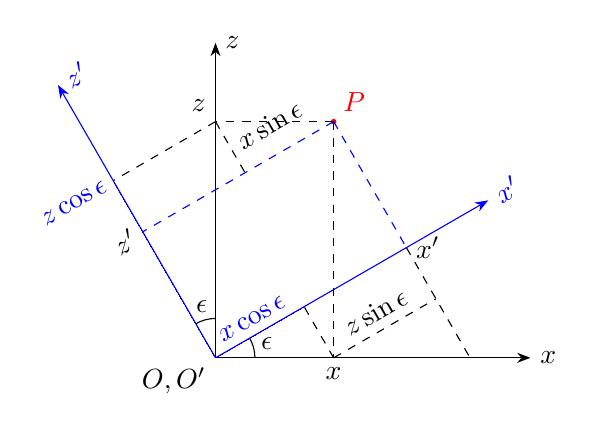
\begin{tikzpicture}[>=Stealth]
        \draw (0,0) node[anchor=north east] {$O,O'$};
        \draw[->] (0,0) -- (4,0) node[anchor=west]{$x$};
        \draw[->] (0,0) -- (0,4) node[anchor=west]{$z$};
        \draw[->,color=blue] (0,0) -- (3.464102,2) node[anchor=west,rotate=30]{$x'$};
        \draw[->,color=blue] (0,0) -- (-2,3.464102) node[anchor=west,rotate=30]{$z'$};
        \fill[radius=1pt,color=red] (1.5,3) circle node[anchor=south west] {$P$};
        \draw[dashed] (1.5,3) -- (1.5,0);
        \draw (1.5,0) node[anchor=north] {$x$};
        \draw[dashed] (1.5,3) -- (0,3);
        \draw (0,3) node[anchor=south east] {$z$};
        \draw[dashed,color=blue] (1.5,3) -- (2.424038,1.399519);
        \draw (2.424038,1.399519) node[anchor=west] {$x'$};
        \draw[dashed,color=blue] (1.5,3) -- (-0.924038,1.600481);
        \draw (-0.924038,1.600481) node[anchor=east,rotate=30] {$z'$};
        \draw (0.5,0) arc [start angle=0,radius=0.5,delta angle=30];
        \draw (0.65,0.175) node {$\epsilon$};
        \draw (0,0.5) arc [start angle=90,radius=0.5,delta angle=30];
        \draw (-0.175,0.65) node {$\epsilon$};
        \draw[dashed] (1.5,0) -- (1.125,0.649519);
        \draw[line width=0,color=blue] (0,0) -- (1.125,0.649519) node[midway,above,rotate=30] {$x\cos\epsilon$};
        \draw[dashed] (2.424038,1.399519) -- (3.232051,0);
        \draw[dashed] (1.5,0) -- (2.799038,0.75) node[midway,above,rotate=30] {$z\sin\epsilon$};
        \draw[dashed] (0,3) -- (-1.299038,2.25);
        \draw[dashed] (0,3) -- (0.375,2.350481) node[midway,right,rotate=30] {$x\sin\epsilon$};
        \draw[line width=0,color=blue] (0,0) -- (-1.299038,2.25) node[left,rotate=30] {$z\cos\epsilon$};
    \end{tikzpicture}
\end{center}

如图，$(x,z)$和$(x',z')$之间还有关系：
\begin{equation}
    \begin{cases}
        & x' = x\cos\epsilon + z\sin\epsilon \\
        & z' = z\cos\epsilon - x\sin\epsilon
    \end{cases}
\end{equation}
又显然有$y=y'$和$r'=r$，代入(1)得：
\begin{equation}
    \begin{cases}
        & \sin\theta'\cos\phi' = \sin\theta\cos\phi\cos\epsilon + \cos\theta\sin\epsilon \\
        & \sin\theta'\sin\phi' = \sin\theta\sin\phi \\
        & \cos\theta' = \cos\theta\cos\epsilon - \sin\theta\cos\phi\sin\epsilon
    \end{cases}
\end{equation}
若取$P$点、$z$轴正半轴与球面交点、$z'$轴正半轴与球面交点连成的三角形为球面三角形，令：
\[
    a = \theta',\quad b = \theta,\quad c = \epsilon,\quad
    A = \pi - \phi,\quad B = \phi'
\]
代入(3)得：
\begin{equation}
    \begin{cases}
        & \sin a\cos B = \cos b\sin c - \cos A\sin b\cos c \\
        & \sin A\sin b = \sin a\sin B \\
        & \cos a = \cos b\cos c + \cos A\sin b\sin c
    \end{cases}
\end{equation}
这就是球面三角基本的三个方程。第一个方程是\textbf{正弦——余弦定理}；第二个方程是球面三角的\textbf{正弦定理}，也可以写成：
\[
    \boxed{
        \frac{\sin a}{\sin A} = \frac{\sin b}{\sin B} = \frac{\sin c}{\sin C}
    }
\]
第三个方程是球面三角\textbf{边的余弦定理}：
\[
    \boxed{
        \cos a = \cos b\cos c + \cos A\sin b\sin c
    }
\]
它的一个推广是\textbf{角的余弦定理}：
\[
    \boxed{
        \cos A = -\cos B\cos C + \cos a\sin B\sin C
    }
\]
如果$A = \dfrac{\pi}{2}$，则有：
\[
    \boxed{
        \cos a = \cos b\cos c
    }
\]
这就是球面直角三角形的\textbf{勾股定理}：斜边的余弦等于直角边余弦的乘积。

当球面三角形的边长$a$、$b$、$c$趋于0时，球面三角形退化为平面三角形，此时有：
\[
    \sin a \to a,\quad \cos a \to 1 - \frac{a^2}{2}
\]
保留到$a^2$项，(4)中的三个方程退化为平面形式：（注意角的正余弦不是小量，不能近似）
\begin{equation}
    \begin{cases}
        & c = a\cos B + b\cos A \\
        & \dfrac{a}{\sin A} = \dfrac{b}{\sin B} \\
        & a^2 = b^2 + c^2 - 2bc\cos A
    \end{cases}
\end{equation}

\newpage
\section{例题}

\subsection{在普吉观测大麦哲伦云（IOAA2017-T1）}

大麦哲伦云（LMC）的坐标为赤经$\alpha = \mathrm{5^h24^m}$，赤纬$\delta = -70^\circ00'$。普吉的地理经度为$\lambda = +98^\circ24'$（东经），纬度为$\phi = +7^\circ53'$（北纬）。已知在世界时2017年1月1日$\mathrm{0^h00^m}$时（$\mathrm{UT+0}$），$0^\circ$经线地方恒星时约为$s_0^* = \mathrm{6^h43^m}$，普吉岛的时区为$\mathrm{UT+7}$。那么在普吉岛2017年里的哪天，可以在当地区时$\mathrm{21^h00^m}$观测到大麦哲伦云上中天？
\bigskip

\paragraph{解：}

大麦哲伦云上中天时，普吉岛的地方恒星时为：
\[
    s = \alpha = \mathrm{5^h24^m}
\]
且区时（东经$105^\circ$线的地方平太阳时）为$\mathrm{21^h00^m}$时，普吉岛的地方平太阳时为：
\[
    T = \mathrm{21^h00^m} - (105^\circ - 98^\circ24') \times \frac{\mathrm{1^h}}{15^\circ} = \mathrm{20^h33^m36^s}
\]
注意恒星时超前于平太阳时，此时地方恒星时与地方平太阳时相差：
\[
    \Delta T = s - T = \mathrm{24^h} + \mathrm{5^h24^m} - \mathrm{20^h33^m36^s} = \mathrm{8^h50^m24^s}
\]
相比于2017年1月1日$\Delta T_0 = s_0^* = \mathrm{6^h43^m}$，中间相差$\mathrm{2^h7^m24^s} = 7644\,\mathrm{s}$，这对应于：
\[
    N = 7644\,\mathrm{s} \times \frac{365.2422\,\mathrm{d}}{86400\,\mathrm{s}} = 32.3\,\mathrm{d}
\]
所求的日期就是2017年1月1日之后的$32$日，即2月2日。

显然，本题的求解过程中忽略了普吉岛和$0^\circ$经线的地方恒星时之差，计算$\Delta T$时用的是普吉岛时间，题目中$\Delta T_0$用的则是$0^\circ$经线时间，但同一天内不同时区的$\Delta T$相差极小，对本题答案的影响可以忽略。

\subsection{日出（CNAO2014-T18）}

假定地球围绕太阳做匀速圆周运动。不考虑一天之内太阳的赤道坐标和黄道坐标变化，以及真太阳和平太阳的时差。不考虑观测地的海拔因素、大气折射和太阳的视面积大小。黄赤交角为$\epsilon = 23.44^\circ$。
\begin{enumerate}
    \item[(1)] 计算夏至日北回归线上某地日出点偏离正东方向（从北点起算，方位角$90^\circ$）的角度。
    \item[(2)] 山东成山头的地理经度为$\lambda = +122.71^\circ$（东经），纬度为$\phi = +37.40^\circ$（北纬）。计算夏至日这里的日出时间（北京时间，时区为$\mathrm{UT+8}$）。
\end{enumerate}
\bigskip

\paragraph{解：}
\begin{enumerate}
    \item[(1)]
    如图1，
    \[
        \cos(90^\circ - \delta) = \cos(90^\circ - \phi)\cos(90^\circ - h) + \cos A\sin(90^\circ - \phi)\sin(90^\circ - h)
    \]
    日出时太阳的高度角$h = 0^\circ$，则有：
    \[
        \boxed{
            \cos A = \frac{\sin\delta}{\cos\phi}
        }
    \]
    夏至日太阳的赤纬和北回归线的地理纬度都等于黄赤交角$\epsilon$，所以：
    \[
        \cos A = \frac{\sin\epsilon}{\cos\epsilon} = \tan\epsilon = 0.433568
    \]
    故方位角$A = 64.31^\circ$，偏离正东方向的角度：
    \[
        \Delta A = 90^\circ - 64.31^\circ = 25.69^\circ
    \]

    \item[(2)]
    如图1，由球面三角的余弦定理得：
    \[
        \cos(90^\circ - h) = \cos(90^\circ - \phi)\cos(90^\circ - \delta) + \cos t\sin(90^\circ - \phi)\sin(90^\circ - \delta)
    \]
    日出时太阳的高度角$h = 0^\circ$，则有：
    \[
        \boxed{
            \cos t = -\tan\phi\tan\delta
        }
    \]
    代入数据得时角为：
    \[
        t_1 = 109.36^\circ = \mathrm{7^h17^m26^s},\quad
        t_2 = 250.64^\circ = \mathrm{16^h42^m34^s}
    \]
    考虑到太阳上中天时$t_0 = \mathrm{0^h}$，日出时取$t_2 = \mathrm{16^h42^m34^s}$。

    不考虑一天之内太阳的赤道坐标和黄道坐标变化，那么可以用平太阳时近似恒星时，即太阳从日出到上中天转过的角度等于时角之差：
    \[
        \Delta T = \Delta t = t_0 - t_2 = \mathrm{0^h} + \mathrm{24^h} - \mathrm{16^h42^m34^s} = \mathrm{7^h17^m26^s}
    \]
    由太阳上中天的平太阳时$\mathrm{12^h}$得到日出的时间：
    \[
        T = \mathrm{12^h} - \mathrm{7^h17^m26^s} = \mathrm{4^h42^m34^s}
    \]
    最后将成山头的地方平太阳时转换为北京时间（东经$120^\circ$线的地方平太阳时），即为：
    \[
        T_0 = \mathrm{4^h42^m34^s} - (122.71^\circ - 120^\circ) \times \frac{\mathrm{1^h}}{15^\circ} = \mathrm{4^h31^m44^s}
    \]

    如果按照恒星时转换为平太阳时的标准做法（秋分时两者重合），计算得到的是$T'_0 = \mathrm{4^h42^m21^s}$。

\end{enumerate}

\subsection{海难（IOAA2017-T12）}

遇到海难之后你来到了一个岛上。幸运的是你带着手表，它显示着曼谷时区的时间。你还有一个指南针，一个星图以及一个计算器。你失去了意识，醒来后发现天已经黑了。不幸的是天空中阴云密布。一小时或更久之后你在云缝中看到了猎户座。你估计出了参宿七的地平高度为$h = 52^\circ30'$，利用指南针你测量出了它的方位角为$A = 109^\circ$，这是从北点起算。这时手表显示的时间为2017年11月21日$\mathrm{1^h00^m}$。并且世界时2017年1月1日$\mathrm{0^h00^m}$时（$\mathrm{UT+0}$），$0^\circ$经线地方恒星时约为$s_0^* = \mathrm{6^h43^m}$。参宿七的赤经为$\alpha = \mathrm{5^h15^m}$，赤纬为$\delta = -8^\circ11'$，曼谷的时区为$\mathrm{UT+7}$。
\begin{enumerate}
    \item[(a)] 计算观测时参宿七的时角$t$；
    \item[(b)] 计算观测时的$0^\circ$经线地方恒星时$s^*$；
    \item[(c)] 计算这个岛的地理经度$\lambda$；
    \item[(d)] 计算这个岛的地理纬度$\phi$，精确到角分。
\end{enumerate}
\bigskip

\paragraph{解：}
\begin{enumerate}
    \item[(a)]
    如图，由球面三角的正弦定理得：
    \[
        \frac{\sin(90^\circ - h)}{\sin(t')} = \frac{\sin(90^\circ - \delta)}{\sin(A)}
    \]
    即：
    \[
        t' = \arcsin\left(\frac{\sin A\cos h}{\cos\delta}\right) = 35^\circ33'26'
    \]
    由于时角是逆时针（从北天极向南天极看）计量的，实际的时角$t$应为：
    \[
        t = 360^\circ - t' = 324^\circ26'34' = \mathrm{21^h37^m46^s}
    \]

    \item[(b)]
    由题意，观测时曼谷的区时为2017年11月21日$\mathrm{1^h00^m}$，则此时$0^\circ$经线地方平太阳时为2017年11月20日$\mathrm{18^h00^m}$，距离2017年1月1日$\mathrm{0^h00^m}$有$323.75$日。

    因为一个回归年中恒星日比太阳日多一日，即$365.2422$太阳日对应$366.2422$恒星日，观测时距离$0^\circ$经线地方恒星时2017年1月1日$\mathrm{6^h43^m}$为：
    \[
        \Delta s^* = 323.75\,\mathrm{d} \times \frac{366.2422}{365.2422} = 324.636398\,\mathrm{d}
    \]
    而$0.636398\,\mathrm{d} = \mathrm{15^h16^m25^s}$，故观测时的$0^\circ$经线地方恒星时为：
    \[
        s^* = \mathrm{6^h43^m} + \mathrm{15^h16^m25^s} = \mathrm{21^h59^m25^s}
    \]

    \item[(c)]
    观测时参宿四在这个岛的时角满足$s = \alpha + t$，其中$s$为该岛的地方恒星时，则：
    \[
        s = \alpha + t = \mathrm{5^h15^m} + \mathrm{21^h37^m46^s} - \mathrm{24^h} = \mathrm{2^h52^m46^s}
    \]
    该岛与$0^\circ$经线的地方恒星时之差为：
    \[
        \Delta s = s - s^* = \mathrm{2^h52^m46^s} + \mathrm{24^h} - \mathrm{21^h59^m25^s} = \mathrm{4^h53^m21^s}
    \]
    与平太阳时一样，恒星时差$\mathrm{1^h}$，经度相差$15^\circ$，所以经度差为：
    \[
        \Delta\lambda = \mathrm{4^h53^m21^s} \times \frac{15^\circ}{\mathrm{1^h}} = 73^\circ20'22''
    \]
    该岛的经度为东经$73^\circ20'22''$。

    \item[(d)]
    由球面三角的余弦定理得：
    \[
        \cos(90^\circ - \delta) = \cos(90^\circ - \phi)\cos(90^\circ - h) + \cos(A)\sin(90^\circ - \phi)\sin(90^\circ - h)
    \]
    即：
    \[
        \sin\delta = \sin\phi\sin h + \cos A\cos\phi\cos h
    \]
    令：
    \[
        X=\sin h = 0.793353,\quad
        Y=\cos A\cos h = -0.198193,\quad
        Z = \sin\delta = -0.142341
    \]
    则化为：
    \[
        Z = X\sin\phi + Y\cos\phi
    \]
    这可以用辅助角公式化简得到：
    \[
        Z = \sqrt{X^2 + Y^2}\sin(\phi + \Delta\phi),\quad \Delta\phi = \arctan{\frac{Y}{X}}
    \]
    得到该岛的地理纬度为：
    \[
        \phi = \arcsin{\frac{Z}{\sqrt{X^2 + Y^2}}} - \arctan{\frac{Y}{X}} = \mathrm{4^\circ00'}
    \]
    即北纬$4^\circ00'$。
\end{enumerate}

\subsection{航线的最南点（IOAA2015-T15）}

一架飞机从秘鲁首都利马（Lima）飞往印度尼西亚的日惹（Yogyakarta）。飞机选择了最短的航线，请计算航线上最南点$P$的纬度。已知利马的地理经度为$\lambda_L = -77^\circ1'$（西经），纬度为$\phi_L = -12^\circ2'$（南纬）；日惹的地理经度为$\lambda_Y = 110^\circ26'$（东经），纬度为$\phi_Y = -7^\circ47'$（南纬）。

\begin{center}
    \tdplotsetmaincoords{100}{270}
    \begin{tikzpicture}[scale=3,tdplot_main_coords,>=Stealth]
        \shade[tdplot_screen_coords,ball color = white] (0,0) circle (1);
        \coordinate (O) at (0,0,0);
        \tdplotsetcoord{L}{1}{90}{-50};
        \tdplotsetcoord{Y}{1}{90}{60};
        \tdplotsetcoord{N}{1}{0}{0};
        \tdplotsetcoord{S}{1}{180}{0};
        \tdplotsetcoord{P}{1}{90}{10};
        \draw (L) node[right] {$L$};
        \draw (Y) node[left] {$Y$};
        \draw (N) node[above] {$N$};
        \draw (S) node[below] {$S$};
        \draw (P) node[anchor=south west] {$P$};
        \tdplotdrawarc{(0,0,0)}{1}{-50}{60}{}{};
        \tdplotsetthetaplanecoords{-50};
        \tdplotdrawarc[tdplot_rotated_coords]{(0,0,0)}{1}{0}{180}{}{};
        \tdplotsetthetaplanecoords{60};
        \tdplotdrawarc[tdplot_rotated_coords]{(0,0,0)}{1}{0}{180}{}{};
        \tdplotsetthetaplanecoords{10};
        \tdplotdrawarc[tdplot_rotated_coords]{(0,0,0)}{1}{0}{180}{}{};
    \end{tikzpicture}
\end{center}
\bigskip

\paragraph{解：}

首先证明：如果$P$是轨迹的最南点，则从南极$S$到$P$的大圆弧与飞机航线（大圆弧$YL$）垂直，且通过北极$N$，即大圆弧$SP$就是$P$所在经线的一部分。证明如下：

由于经过南极的大圆弧一定经过南极的对跖点（位于球直径两端的点），也就是北极点，所以从南极$S$到$P$的大圆弧也会通过北极$N$，即大圆弧$SP$就是$P$所在经线的一部分。

在球面三角形$YSP$中，由正弦定理得：
\[
    \frac{\sin y}{\sin Y} = \frac{\sin p}{\sin P}
\]
而$y$、$p$分别是$P$点、$Y$点纬度绝对值的余角，如果$P$是航线上的最南点，则要求$y$达到极小值，即：
\[
    \sin y = \frac{\sin p\sin Y}{\sin P}
\]
达到极小值。

另一方面，$p$是常数，$Y$也是常数（因为球面三角形$YLS$是固定的），所以$\sin p\sin Y$是常数。当$P=90^\circ$时，大圆弧$SP$与大圆弧$YL$垂直，$\sin P$达到最大值，$\sin y$则达到极小值，$y$达到极小值。

在三角形$YSL$中，我们有：
\[
    \widearc{YS} = 82^\circ13',\quad \widearc{LS} = 77^\circ58',\quad \angle YSL = (180^\circ - 77^\circ1') + (180^\circ - 110^\circ26') = 172^\circ33'
\]
根据余弦定理求弧$\widearc{YL}$：
\[
    \cos(\widearc{YL}) = \cos(\widearc{YS})\cos(\widearc{LS}) + \sin(\widearc{YS})\sin(\widearc{LS})\cos(\angle YSL)
\]
得到$\widearc{YL} = 158^\circ50'39''$。

再用余弦定理求角$Y=\angle LYS$：
\[
    \cos(\widearc{LS}) = \cos(\widearc{YS})\cos(\widearc{YL}) + \sin(\widearc{YS})\sin(\widearc{YL})\cos(\angle LYS)
\]
得到$Y = 20^\circ34'16''$。

最后由：
\[
    \sin y = \frac{\sin p\sin Y}{\sin P} = \sin p\sin Y
\]
得$y = 20^\circ22'23''$，则$P$点的纬度为$-90^\circ + 20^\circ22'23'' = -69^\circ37'37''$（南纬）。

\newpage
\section{练习题}

1. 已知黄赤交角为$\epsilon=23^\circ26'$，黄白交角为$\psi=5^\circ9'$，如果八意永琳在幻想乡持续观测月亮的升起并记录升起时的方位角，方位角最大值与最小值之差为多少？幻想乡的地理纬度为$\phi = +39^\circ59'$（北纬），忽略大气折射和黄白交角的波动。（答案：$77^\circ16'36''$）
\bigskip

2. 接例题4，计算航线上最南点$P$的经度。（答案：西经$162^\circ28'33''$）
\bigskip

3. 由于地球的岁差，有没有可能在一个时间，天狼星永远不会从波兰克拉科夫升起，而老人星会升起和落下？黄赤交角为$\epsilon=23^\circ26'$，克拉科夫的纬度为$\phi = +50^\circ6'$（北纬）。天狼星的赤经$\alpha_1=\mathrm{6^h45^m}$，赤纬$\delta_1=-16^\circ43'$；北银极的赤经$\alpha_2=\mathrm{6^h24^m}$，赤纬$\delta_2=-52^\circ42'$。（IOAA2011-T12）
\bigskip

4. 黄道圈在赤道坐标系$(\alpha,\delta)$下的方程有这样的形式：
\[
    \delta = \arctan(\sin\alpha\tan\epsilon)
\]
其中$\epsilon$为黄赤交角。对于纬度在$\phi = +49^\circ34'$（北纬）、地方恒星时为$s = \mathrm{0^h51^m}$的观测者，找出银道圈在地平坐标系$(A,h)$下类似的方程形式$h = f(A)$。北银极的赤经$\alpha^*=\mathrm{12^h51.4^m}$，赤纬$\delta^*=27^\circ8'$。（IOAA2011-T13）
\bigskip

5. 假设有一个使徒正好站在南极圈上，定义地平面上的直角坐标系$Oxy$，原点$O$为使徒的基座，$x$轴为东西方向，$y$轴为南北方向。在南半球，太阳高挂的某个“至日”那天使徒的影长最短，忽略太阳当日赤纬方向的移动，写出描述使徒顶端在地平面投影所画出的圆锥曲线的方程。忽略大气折射，黄赤交角为$\epsilon=23^\circ26'$，使徒的高度为$H=39.60\,\mathrm{m}$。（IOAA2012-T15）
\bigskip


\end{document}